\chapter{Оцінка даних}\label{cha:basic_data_exploration}
Першим кроком у будь-якому проекті машинного навчання є ознайомлення з даними.
Для цього ви будете використовувати бібліотеку Pandas.
Pandas - основний інструмент даних, який вчені використовують для вивчення та обробки даних.
Більшість людей скорочують панд у своєму коді як pd.
Ми робимо це за командою

\begin{lstlisting}[style=light, language=Python,label={lst:vectorimg},caption=Імпортування Pandas]
import pandas as pd
\end{lstlisting}

Найважливішою частиною бібліотеки Pandas є \textbf{DataFrame}.
DataFrame містить тип даних, яку ми можемо сприймати як таблицю.
Це схоже на аркуш у Excel або таблицю в базі даних SQL.

Як приклад, ми розглянемо дані про ціни на житло в Айові.

Приклади даних (Айові) знаходяться на шляху до файлу ../input/melbourne-housing-snapshot/train.csv.

Ми завантажуємо та досліджуємо дані за допомогою таких команд:

\begin{lstlisting}[style=light, language=Python,label={lst:vectorimg},caption=Імпортування Pandas]
import pandas as pd

# Path of the file to read
iowa_file_path = '../input/home-data-for-ml-course/train.csv'

# Fill in the line below to read the file into a variable home_data
c = pd.read_csv(iowa_file_path)

home_data = pd.read_csv(iowa_file_path)
home_data.describe()

\end{lstlisting}

\begin{figure}
    \label{fig:data_iowa}
    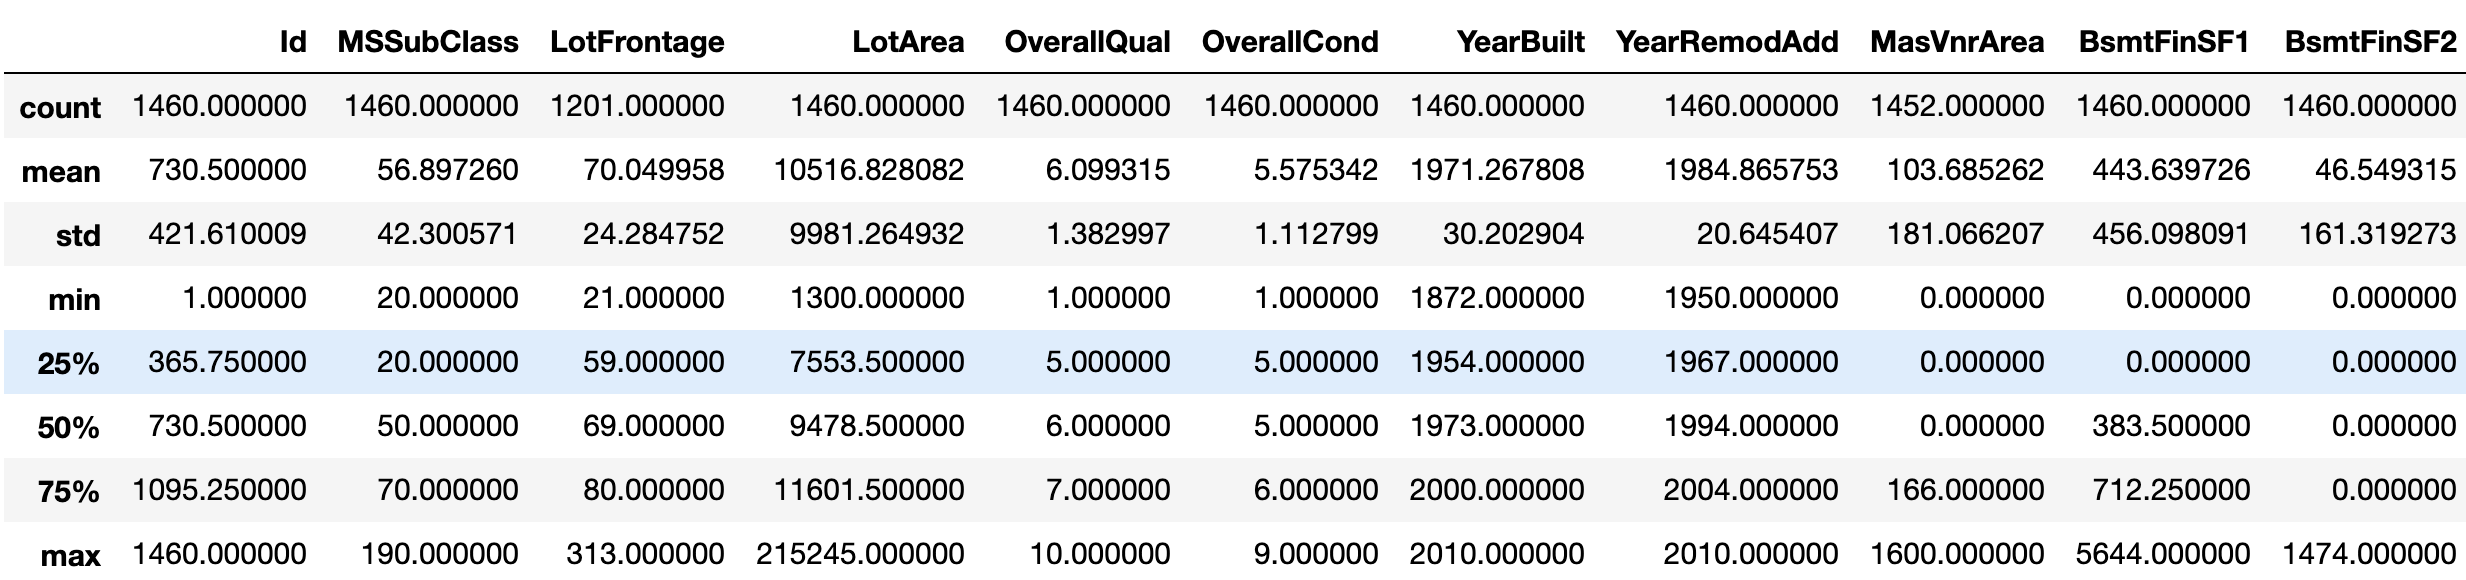
\includegraphics[scale=0.4]{data-iowa.png}

    Результат виконаня команди describe()
\end{figure}

\section{Опис даних}\label{sec:data_description}
Результати показують 8 чисел для кожного стовпця у вихідному наборі даних.
Перше число, \textbf{count}, показує, скільки рядків мають невідсутні значення.

Відсутні цінності виникають з багатьох причин.
Наприклад, розмір 2-ї спальні не буде збиратися при обстеженні 1-кімнатного будинку.
Ми повернемось до теми відсутніх даних.

Друге значення - \textbf{mean}, яке є середнім значенням.
Під цим, \textbf{std} - це стандартне відхилення, яке вимірює, наскільки чисельно розподілені значення.

Щоб інтерпретувати значення min, \textbf{25\%, 50\%, 75\%} та max, уявіть, як сортуватиме кожен стовпець від найнижчого до найвищого значення.
Перше (найменше) значення - це мін.
Якщо ми пройдемо чверть шляху по списку, ми знайдемо число, яке перевищує 25\% значень і менше 75\% значень.
Це значення 25\% (вимовляється "25-й процентиль").
50-й та 75-й процентилі визначаються аналогічно, і max - найбільша кількість.

\section{Інтерпретація}\label{sec:interpretation}

Найновштй будинок у наших даних не такий вже й новий.
Кілька можливих пояснень цьому:

\begin{itemize}
    \item В регіоні де збирали дані, не будували нових будинків.
    \item Дані були зібрані давно. Будинки, побудовані після публікації даних, не відображатимуться.
\end{itemize}

Скоріш за все, набір даних застарілий.
Ми можемо перевірити це, порівнявши сьогодні дані про житло в Айові з тими, що перелічені в наборі даних, і побачити останній рік побудови, рік продажу тощо.
Якщо будь-який із них перевищує 2011 рік, ми можемо підтвердити, що набір даних застарілий.

Це проблема, оскільки якщо ми використовуємо цей набір даних для прийняття рішень про купівлю, продаж та залучення на ринок житла в Айові, уявлення, які ми могли б отримати з цих даних, сьогодні, швидше за все, будуть не такими актуальними.

Приклад відмінностей:
\begin{itemize}
    \item Ціна продажу, ймовірно, вища через стабільно зростаючий ринок житла в США.
    \item Більше готових підвалів старих будинків.
    \item Різні особливості будинку можуть мати дещо іншу вагу, ніж 10 років тому.
\end{itemize}
